\documentclass[aspectratio=43,english]{beamer} %If you want to create Polish presentation, replace 'english' with 'polish' and uncomment 3-th line, i.e., '\usepackage{polski}'
\usepackage[utf8]{inputenc}
\usepackage{polski} %Uncomment for Polish language
\usepackage{babel}
\usepackage{listings} %We want to put listings

\mode<beamer>{ 	%in 'beamer' mode
	\hypersetup{pdfpagemode=FullScreen}		%Enable Full screen mode
	\usetheme{JuanLesPins} 		%Show part title in right footer
	%\usetheme[dark]{AGH}                 		%Use dark background
	%\usetheme[dark,parttitle=leftfooter]{AGH}  	%Use dark background and show part title in left footer
}
\mode<handout>{	%in 'handout' mode
	\hypersetup{pdfpagemode=None}		
	\usepackage{pgfpages}
  	\pgfpagesuselayout{4 on 1}[a4paper,border shrink=5mm,landscape]	%show 4 slides on 1 page
  	\usetheme{boxes}
  	\addheadbox{structure}{\quad\insertpart\hfill\insertsection\hfill\insertsubsection\qquad} 	%content of header
 	\addfootbox{structure}{\quad\insertauthor\hfill\insertframenumber\hfill\insertsubtitle\qquad} 	%content of footer
}

\AtBeginPart{ %At begin part: display its name
	\frame{\partpage}
} 


%%%%%%%%%%% Configuration of the listings package %%%%%%%%%%%%%%%%%%%%%%%%%%
% Source: https://en.wikibooks.org/wiki/LaTeX/Source_Code_Listings#Using_the_listings_package
%%%%%%%%%%%%%%%%%%%%%%%%%%%%%%%%%%%%%%%%%%%%%%%%%%%%%%%%%%%%%%%%%%%%%%%%%%%%
\lstset{ %
  backgroundcolor=\color{white},   % choose the background color
  basicstyle=\footnotesize,        % the size of the fonts that are used for the code
  breakatwhitespace=false,         % sets if automatic breaks should only happen at whitespace
  breaklines=true,                 % sets automatic line breaking
  captionpos=b,                    % sets the caption-position to bottom
  commentstyle=\color{green},      % comment style
  deletekeywords={...},            % if you want to delete keywords from the given language
  escapeinside={\%*}{*)},          % if you want to add LaTeX within your code
  extendedchars=true,              % lets you use non-ASCII characters; for 8-bits encodings only, does not work with UTF-8
  frame=single,	                   % adds a frame around the code
  keepspaces=true,                 % keeps spaces in text, useful for keeping indentation of code (possibly needs columns=flexible)
  keywordstyle=\color{blue},       % keyword style
  morekeywords={*,...},            % if you want to add more keywords to the set
  numbers=left,                    % where to put the line-numbers; possible values are (none, left, right)
  numbersep=5pt,                   % how far the line-numbers are from the code
  numberstyle=\tiny\color{gray},   % the style that is used for the line-numbers
  rulecolor=\color{black},         % if not set, the frame-color may be changed on line-breaks within not-black text (e.g. comments (green here))
  showspaces=false,                % show spaces everywhere adding particular underscores; it overrides 'showstringspaces'
  showstringspaces=false,          % underline spaces within strings only
  showtabs=false,                  % show tabs within strings adding particular underscores
  stepnumber=2,                    % the step between two line-numbers. If it's 1, each line will be numbered
  stringstyle=\color{cyan},        % string literal style
  tabsize=2,	                   % sets default tabsize to 2 spaces
  title=\lstname,                  % show the filename of files included with \lstinputlisting; also try caption instead of title
                                   % needed if you want to use UTF-8 Polish chars
  literate={?}{{\k{a}}}1
           {?}{{\k{A}}}1
           {?}{{\k{e}}}1
           {?}{{\k{E}}}1
           {�}{{\'o}}1
           {�}{{\'O}}1
           {?}{{\'s}}1
           {?}{{\'S}}1
           {?}{{\l{}}}1
           {?}{{\L{}}}1
           {?}{{\.z}}1
           {?}{{\.Z}}1
           {?}{{\'z}}1
           {?}{{\'Z}}1
           {?}{{\'c}}1
           {?}{{\'C}}1
           {?}{{\'n}}1
           {?}{{\'N}}1
}
%%%%%%%%%%%%%%%%%


\title{Metody Obliczeniowe w Nauce i Technice}
\author{Marian Bubak, PhD}
\date{}
\institute[AGH]{
	Institute of Computer Science\\ul. Kawiory 21\\30-055 Krakow\\
	Poland\\
	\url{http://www.icsr.agh.edu.pl/~mownit/}
}



%%%%%%%%%%%%%%%%
\usepackage{amsmath}
%%%%%%%%%%%%%%%%

\subtitle{15. Obliczanie całek metodami Monte Carlo}
\setcontributors{Maciej Trzebiński\\Mikołaj Biel}


\begin{document}
	\maketitle
    %%%%%%%%%%%%%%%%
    \begin{frame}{Outline}
    	\tableofcontents
    \end{frame}

    %%%%%%%%%%%%%%%%
    \section{Przegląd zastosowań}
%%%%%%%%%%%%%%%%
\begin{frame}{Przegląd zastosowań}
	\begin{itemize}
		\item Obliczanie całek,
        \item W fizyce - MC to uśrednianie względem zespołu; stosowana zamiast rozwiązywania deterministycznych równań ruchu (co jest uśrednianiem względem czasu); przestrzeń fazowa jest b. wielowymiarowa,
        \item Rozwiązywanie równań różniczkowych cząstkowych - przez wprowadzenie błądzenia przypadkowego,
        \item Symulacje typu ,,transport promieniowania'',
        \item Symulacje typu ,,systemy obsługi masowej''
	\end{itemize}
\end{frame}
    %%%%%%%%%%%%%%%%
    \section{Dlaczego MC i całki?}
%%%%%%%%%%%%%%%%
\begin{frame}{Dlaczego MC i całki?}
	\begin{enumerate}[a)]
		\item
        	$X$ - zmienna losowa ciągła, wartości z $(a, b)$ zgodnie z rozkładem $f(x)$ \\
            $g$ - ustalona funkcja \\
            $y = g(x)$ - zmienna losowa
            
            {\bf Wart. oczekiwana} $Y: E\{Y\} = E\{g(x)\} = \int_a^b g(x) f(x) dx$ \hfill $(*)$
	\end{enumerate}
\end{frame}
%%%%%%%%%%%%%%%%
\begin{frame}{Dlaczego MC i całki?}
	\begin{enumerate}
		\item[b)]
			chcemy obliczyć całkę: $I = \int_a^b h(x) dx$ \\
            niech $f: f(x) > 0$ dla $x \in (a, b), \int_a^b f(x) dx = 1$ \\
            $f(x)$ - gęstość rozkładu pewnej zmiennej losowej przyjmującej wartości z $(a, b)$ \\
            $I = \int_a^b \frac{h(x)}{f(x)} f(x) dx = \int_a^b g(x)f(x)dx$ \hfill $\leftarrow$ całka postaci $(*)$ \\
            Obliczanie całki można zawsze przedstawić jako zagadnienie obliczania wartości oczekiwanej pewnej zmiennej losowej ciągłej.
            \\[8pt]
            (suma szeregu - zmienna losowa dyskretna)
	\end{enumerate}
\end{frame}
    %%%%%%%%%%%%%%%%
    \section{Całkowanie metodą ,,orzeł-reszka''}
%%%%%%%%%%%%%%%%
\begin{frame}{Całkowanie metodą ,,orzeł-reszka''}
	Szukamy $I = \int_0^1 f(x) dx; 0 \le f(x) \le 1$
    
    {\centering 
    	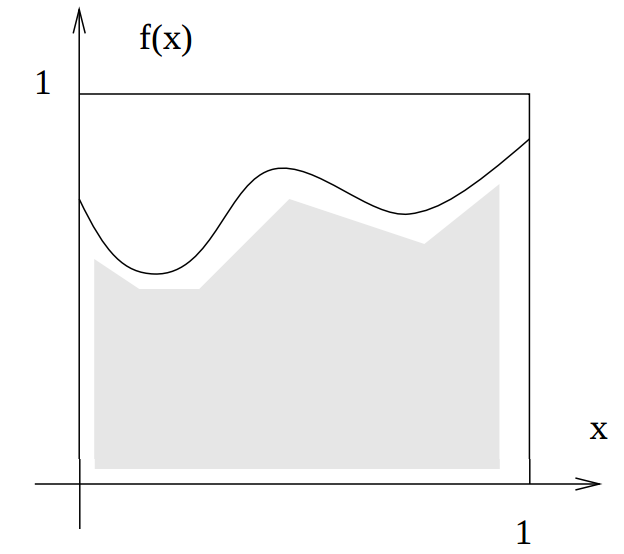
\includegraphics[width=.4\linewidth]{img/15/15_1_orzel_reszka}
        \par
    }
    
    $(X, Y)$ - dwuwymiarowa zmienna losowa o rozkładzie równomiernym na kwadracie: $(0 \le x \le 1, 0 \le y \le 1)$ \\
    Prawdopodobieństwo, że $(X, Y)$ przyjmie wartość z zakreskowanej części rysunku jest równe tej powierzchni, czyli wartości całki $I$.
\end{frame}
%%%%%%%%%%%%%%%%
\begin{frame}{Metoda}
	$N$ - eksperymentów: obserwacji $(X, Y)$ \\
    $M$ - liczba eksperymentów, w których $(X, Y)$ poniżej $f(x)$
    \\[8pt]
    Jeżeli obserwacje niezależne - to $M$ ma rozkład dwumianowy
    
    \[\boxed{
    	P\{M = m\} = \left(
            \frac{N}{m}
        \right) I^m (1-I)^{N-m}
    }\]
\end{frame}
%%%%%%%%%%%%%%%%
\begin{frame}{Metoda}
	Zadanie:\\
    oszacowanie $\hat{I} = \frac{M}{N}$ \\
    wariancja $S^2(\hat{I}) = \frac{1}{N} \frac{M}{N} \left( 
    	1 - \frac{M}{N}
    \right)$ 
    \\[8pt]
    Metoda:
    \begin{itemize}
    	\item prosta,
        \item łatwe uogólnienie na n-D
        \item mało efektywna
    \end{itemize}
\end{frame}
    %%%%%%%%%%%%%%%%
    \section{Metoda podstawowa}
%%%%%%%%%%%%%%%%
\begin{frame}{Metoda podstawowa}
	\[
    	I = \int_a^b f(x) dx = \int_a^b h(x)g(x) dx = E\{Y\}
    \]
    $g(x)$ - gęstość pewnej zmiennej losowej $X \in (a, b)$
    
    Np.:
    \begin{itemize}
    	\item $Y = h(x)$
        \item $I = (b-a) \int_a^b f(x) \underbrace{\frac{dx}{b-a}}_\text{dP}$, $P$ - rozkład równomierny na $(a, b)$
    \end{itemize}
    
\end{frame}
%%%%%%%%%%%%%%%%
\begin{frame}{Metoda podstawowa}
    Bez utraty ogólności wystarczy rozpatrywać: \[
    	I = \int_0^1 f(x) dx = E\{Y\}
    \]
    $Y = f(X)$, przy czym $X$ - zmienna losowa o rozkładzie równomiernym $(0, 1)$
    
    Oszacowanie $E\{Y\}$ - średnia z $N$ niezależnych obserwacji: \[
    	\boxed{
        \hat{I} = \frac{1}{N} \sum_{i=1}^n f(x_i) \hspace{.5cm} (**)
        }
    \]
\end{frame}
%%%%%%%%%%%%%%%%
\begin{frame}{Metoda podstawowa - procedura}
    \begin{block}{Procedura}
        \begin{enumerate}
            \item wylosować $x_1, x_2, ..., x_N$ wg rozkładu równomiernego na $(0, 1)$
            \item obliczyć $f(x_1), f(x_2), ..., f(x_N)$
            \item średnia $(**)$
        \end{enumerate}
    \end{block}
\end{frame}
%%%%%%%%%%%%%%%%
\begin{frame}{Metoda podstawowa - wariancja}
	\vspace{-.5cm}
	\begin{block}{Wariancja}
		\begin{align*}
			\sigma^2(\hat{I}) = 
            \sigma^2 \frac{1}{N} \left[ 
            	\sum_{i=1}^n f(x_i)
            	\right] =
            \frac{1}{N^2} \sum_{i=1}^N \sigma^2 [f(x_i)] =
            \\
            \frac{1}{N} \sigma^2 [f(x)] = 
            \frac{1}{N} \left[ 
            	\int_0^1 f^2(x)dx - I^2
            	\right]
		\end{align*}
	\end{block}
    
    \begin{block}{Estymator wariancji}
    	\[
        	\sigma^2(\hat{I}) = \frac{1}{N} \sigma_f^2; 
            \sigma_f^2 = \frac{1}{N-1} \sum_{i=1}^N [f(x_i) - \hat{I}]^2
        \]
    \end{block}
    
    $\sigma^2(\hat{I}_1) - \sigma^2(\hat{I}_2) > 0$ \hspace{.5cm}
    1 - orzeł/reszka; \hspace{.5cm}
    2 - podstawowa
\end{frame}
    %%%%%%%%%%%%%%%%
    \section{Metoda średniej ważonej ({\it importance sampling})}
%%%%%%%%%%%%%%%%
\begin{frame}{Metoda średniej ważonej}
	$f(x) = const.$ - w met. podstawowej - poj. punkt to wynik dokładny \\
    stąd: $f(x)$ - gładkie - liczba losowań - mała
    \\[8pt]
    Met. średniej ważonej - $g(x)$ - ciągła, $x \in [0, 1]$:
    \begin{enumerate}
    	\item $g(x) > 0, x \in [0, 1]$
        \item $\int_0^1 g(x) dx = 1$
        \item $\frac{f(x)}{g(x)}, x \in (0, 1)$ - znacznie gładsza niż $f(x)$
        \item $g(x)$ - dana prostym wzorem analitycznym
    \end{enumerate}
    
    \[
    	\left.
        	\begin{array}{ll}
        		\text{1, 2 - precyzyjne} \\
        		\text{3, 4 - rozmyte}
        	\end{array}
        \right\} 
        \text{warunki}
    \]
\end{frame}
%%%%%%%%%%%%%%%%
\begin{frame}{Metoda średniej ważonej - dygresja}
	\begin{block}{Dygresja - sugestia, co do dobrego $g(x)$}
		$X$ - zmienna losowa, \\
        $G(x)$ - dystrybuanta X; $G(x) = P(X < x)$
        \\[8pt]
        niech $G(x)$ - funkcja ściśle rosnąca: \[
        	P[\underbrace{G(x)}_\eta < \underbrace{G(x')}_{\eta'}] = P(x < x') = \underbrace{G(x')}_{\eta'}
        \]
        
        {\bf wniosek:} Jeżeli zmienna losowa $X$ ma ściśle rosnącą dystrybuantę $G(x)$, to $G(x)$ ma rozkład równomierny na $(0, 1)$
	\end{block}
\end{frame}
%%%%%%%%%%%%%%%%
\begin{frame}{Metoda średniej ważonej - dygresja}
	\begin{block}{Dygresja - sugestia, co do dobrego $g(x)$}
    	... stąd - sposób obliczania $I = \int_0^1 f(x) dx$:
        \begin{enumerate}
        	\item $g_1(x) > 0$ - 1-sza propozycja,
            \item dobór stałej - $g(x) = \alpha g_1(x); \alpha \int_0^1 g_1(x) dx = 1$
            \item analitycznie: $G(x) = \int_0^x g(x') dx'$
            \item losujemy z rozkładem równomiernym: $y_1 \in (0, 1), i = 1, ..., N$
            \item rozwiązujemy $G(x_i) = y_i \Rightarrow x_i, i = 1, ..., N$
            \item przybliżona wartość całki: $I \approx \frac{1}{N} \sum_{i=1}^N f(x_i)$
        \end{enumerate}
	\end{block}
\end{frame}
%%%%%%%%%%%%%%%%
\begin{frame}{Metoda średniej ważonej - dygresja}
	\begin{block}{Dygresja - sugestia, co do dobrego $g(x)$}
    	\centering 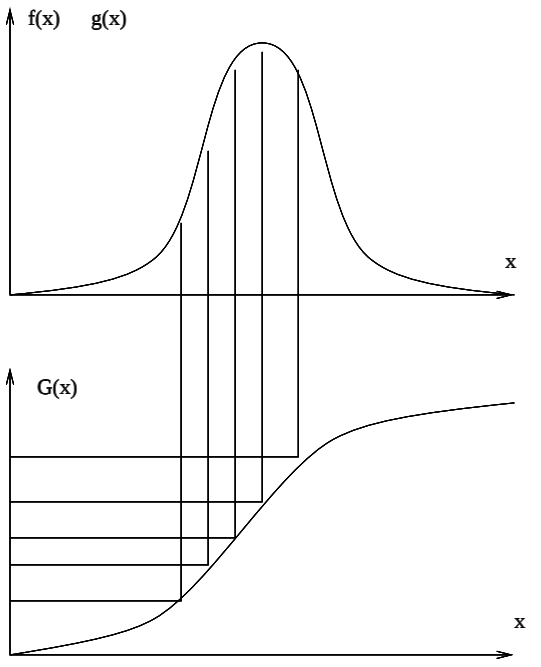
\includegraphics[width=.4\linewidth]{img/15/15_2_dobre_gx}
	\end{block}
\end{frame}
    %%%%%%%%%%%%%%%%
    \section{Literatura}
%%%%%%%%%%%%%%%%
\begin{frame}[allowframebreaks]{Literatura}
	\begin{thebibliography}{9}
		\setbeamertemplate{bibliography item}[book]
            \bibitem{zielinski}{R. Zieliński \newblock Metody Monte Carlo \newblock WNT, 1970 }
		\setbeamertemplate{bibliography item}[book]
            \bibitem{jermakow}{S.M. Jermakow \newblock Metoda Monte Carlo i zagadnienia pokrewne \newblock PWN 1976 }
		\setbeamertemplate{bibliography item}[book]
            \bibitem{hammersley}{J.M. Hammersley, D.C. Handscomb \newblock Monte Carlo Methods \newblock 1964 }
		\setbeamertemplate{bibliography item}[book]
            \bibitem{spanier}{J. Spanier, E.M. Gelbard \newblock Monte Carlo principles and transport problems \newblock Addison - Wesley, 1969 }
		\setbeamertemplate{bibliography item}[book]
            \bibitem{binder1}{K. Binder (Ed.) \newblock Monte Carlo Methods in Statistical Physics \newblock Springer - Verlag, 1979 }
		\setbeamertemplate{bibliography item}[book]
            \bibitem{binder2}{K. Binder (Ed.) \newblock Applications of the MC Methods in Statistical Physics \newblock Springer - Verlag, 1984 }
		\setbeamertemplate{bibliography item}[book]
            \bibitem{binder3}{K. Binder \newblock Applications of the MC Methods in Statistical Physics; Topics in Current Physics \newblock Springer - Verlag, 1987 }
		\setbeamertemplate{bibliography item}[book]
            \bibitem{knuth}{D.E. Knuth \newblock The Art of Computer Programming, vol. 2: Seminumerical Algorithms \newblock Addison - Wesley, 1981 }
		\setbeamertemplate{bibliography item}[book]
            \bibitem{kalos}{M.H. Kalos, P.A. Whitlock \newblock Monte Carlo Methods \newblock Wiley, New York, 1986 }
		\setbeamertemplate{bibliography item}[book]
            \bibitem{bratley}{P. Bratley, B.L. Fox, E.L. Schrage \newblock A Guide to Simulation \newblock Springer Verlag, New York, 1983 }
	\end{thebibliography}
\end{frame}
    %%%%%%%%%%%%%%%%

\end{document}
